% Generated from: Zhihu/专栏：概率与统计/渐近统计 (11)：Bootstrap（下）_金鱼马_2026-08-03.md
% 在上一篇中，我们主要讨论了 Bootstrap 的一些理论上的渐近性质，包括一阶正确性和二阶有效性。

% 本篇简单讨论如何将 Bootstrap 应用于置信区间等统计推断问题。关于 Bootstrap 的应用，也可参考 Davison 与 Hinkley~\cite{davisonhinkley1997}。

\section{Bootstrap 置信区间}

\subsection{回顾区间估计}

枢轴量法可以说是寻找置信区间的一个比较一般的方法。

样本 $X=(X_1,\dots,X_n)$ 取自于总体 $P$ ， $\theta$ 是该总体的参数：可以是有限的，也可以是一个统计泛函 $\theta=\theta(P)$ ，这里我们只考虑总体和参数均是一维的情形。假设存在样本 $X$ 和参数 $\theta$ 的一个函数 $R_n(X;\theta)$ ，称作\textbf{\emph{根}} (root)，其分布已知，则对于任给的 $0<\alpha<1$ ，可找到区间 $[c(\theta),d(\theta)]$ 使得

\begin{equation}
\label{eq:ch11b:tag-5}
P\big(c(\theta)\le R_n(X;\theta)\le d(\theta)\big)\ge 1-\alpha,\quad \forall\theta
\end{equation}

如果对固定的 $X$ ，能通过 $c(\theta)\le R_n(X;\theta)\le d(\theta)$ 反解出 $\theta$ 的范围 $C_n(X)=\{\theta:c(\theta)\le R_n(X;\theta)\le d(\theta)\}$，且这个范围总是一个有限区间，则 $C_n$ 就是 $\theta$ 的一个 $1-\alpha$ 置信区间。

区间 $[c(\theta),d(\theta)]$ 有很多种选取方法，当其分布比较简单时，可以考虑\emph{最高概率密度区间 }(highest density interval, HDI)，使得区间长度最短；也可以取\emph{等尾置信区间} (equal-tailed interval, ETI)，即让 \[ P(R_n(X;\theta)<c(\theta))=P(R_n(X;\theta)>d(\theta))=\frac\alpha2 \]此时， $c(\theta),d(\theta)$ 分别是 $R_n(X;\theta)$ 分布的 $\tfrac\alpha2$ 和 $1-\tfrac\alpha2$ 分位数，并且这样得来的置信区间是精确的。

如果有 $\theta$ 的一个良好的点估计 $\widehat\theta_n=\widehat\theta_n(X)$ ，那么它是最有可能接近真参数 $\theta$ 的，围绕 $\widehat\theta_n$ 的区间，包含真参数值的可能性也就要大一些。因此， $R_n(X;\theta)=R_n(\widehat\theta_n(X),\theta)$ 经常通过估计量 $\widehat\theta_n$ 构建，这也更加方便。

如果 $R_n(X;\theta)$ 的分布不依赖于 $P$ ，则 $c(\theta)\equiv c$ 、 $d(\theta)\equiv d$ 均可取为常数，此时称 $R_n(X;\theta)$ 为\textbf{\emph{枢轴量}} (pivotal quantity)；除了少数情况，找到枢轴量可能很困难，传统上往往用大样本方法，找到某个根 $R_n(X;\theta)$ 在 $n\to\infty$ 时候的渐近分布不依赖于 $\theta$ ，此时称 $R_n(X;\theta)$ 是\textbf{\emph{渐近枢轴量 }} (asymptotic pivotal)；用渐近分布来替代 $R_n(X;\theta)$ 本身的分布构建有关参数的置信区间 $C_n(X)$ ，使得
\[\liminf_{n\to\infty}P(\theta\in C_n(X))\ge 1-\alpha\]
则称 $C_n$ 有渐近覆盖 $1-\alpha$ 。

\begin{remark}
注意区分：``枢轴量''要求其分布不依赖未知参数；``根''可以是任意关于 $X$ 和 $\theta$ 的函数，无论其分布是否依赖 $\theta$。``根''这一称呼来自 \cite{beran1987}。
\end{remark}

参数属于置信区间的概率 $P(\theta\in C_n(X))$ ，即式~\eqref{eq:ch11b:tag-5} 左侧的值，称作``\textbf{\emph{真实覆盖 }} (true coverage)''；而式~\eqref{eq:ch11b:tag-5} 右侧的 $1-\alpha$ 是预先取定的，称之为``\textbf{\emph{名义覆盖 }} (nominal coverage)''或者``名义水平 (nominal level)''。若水平和覆盖概率恰好相同，则称该区间是\textbf{\emph{精确}} (exact) 的。 $R_n(X;\theta)$ 的分布可能很复杂，难以找到精确置信区间，我们将真实覆盖与名义覆盖的差值
\[P(\theta\in C_n(X))-(1-\alpha)\]
称作\textbf{\emph{覆盖误差}} (Coverage error)：它衡量的是置信区间有多准，如果覆盖误差正向过大，说明 $C_n(X)$ 过于保守；若为较大负值则反而覆盖不足。最好这个误差能够随着 $n\to\infty$ 越来越接近 0，从而区间越来越接近精确。因此定义

\begin{itemize}
\tightlist
\item
  \textbf{\emph{一阶正确}} ：当 $n\to\infty$时， $P(\theta_0\in C_n)\to 1-\alpha$ ；
\item
  \textbf{\emph{二阶准确}} ： $P(\theta_0\in C_n)=1-\alpha+O(n^{-1})$ 。
\end{itemize}

Bootstrap 方法可以用来尽可能缩减覆盖误差、给出更精确的置信区间。这是因为，要想构造置信区间，就说明我们需要对根 $R_n(X;\theta)$ 的确切分布是已知的，或者至少要知道它的分位数；若未知，那么必须对其进行估计。Bootstrap 正好能够提供尽可能准确的估计。

本节最后，举一个经典的置信区间例子。

\begin{example}[Wald 置信区间]\label{ex:ch11:wald}

设有 $X_1,\dots,X_n\sim P$i.i.d.，其中 $P$ 是某个一维连续分布，方差 $0<\sigma^2<\infty$ 。要做统计泛函
\[
\theta(P)=\mathbb E_P[X]=\int_{\mathbb R}x\mathrm dP(x)
\]

的区间估计，可取
\[
R_n(X;\theta):=\frac{\bar X_n-\theta}{\widehat{\mathrm{se}}_n}\overset{\rm d}\to \mathcal N(0,1).
\]

其中 $\widehat{\mathrm{se}}_n$ 是样本标准误，它是总体标准误 $\mathrm{se}=\sigma/\sqrt n$ 的相合估计，常取 $\widehat{\mathrm{se}}_n=\sqrt{\frac1{n(n-1)}\sum_{j=1}^n(X_j-\bar X_n)^2}$ 。

将 $\mathcal N(0,1)$ 近似 $R_n(X;\theta)$ 的分布，即可得到渐近 $\mathcal N(0,1)$ 置信区间，称作 \textbf{\emph{Wald置信区间}} ： \[ C_n^{\text{Wald}}=\Big[\bar X_n-z_{1-\alpha/2}\widehat{\mathrm{se}}_n,\bar X_n+z_{1-\alpha/2}\widehat{\mathrm{se}}_n\Big] \]其中 $z_{1-\alpha/2}=\Phi^{-1}(\alpha/2)$ 是 $\mathcal N(0,1)$ 的 $1-\tfrac\alpha2$ 分位数，它是一阶准确的。

例如，常取 $\alpha=5\%$ ， $z_{1-\alpha/2}\approx -1.96$ ，那么近似 95\% 置信区间就是 $\bar X_n\pm1.96\ \widehat{\mathrm{se}}_n$ 。

当然这个方法在固定的 $n$ 下并不很准确。举一个例子，对 $\mathrm{Poisson}(\theta)$ 分布，从 $\mathrm{Poisson}(\theta)$ 中抽取出一个样本 $X=10$ 时，使用 Wald 置信区间计算得到 $[3.8,16.2]$ ，但是精确的等尾置信区间却是 $[5.1,17.8]$ 。两种方法的计算细节如下：

\begin{itemize}
\tightlist
\item
  Wald 置信区间用 $\widehat{\mathrm{se}}_n=\sqrt {\bar X_n}/\sqrt n$ 计算，这是利用了 Poisson 分布的特殊性质：均值和方差相等；取 $n=1$ 、 $\bar X_1=X=10$ ，得到 $C_n^{\text{Wald}}=[10-1.96\sqrt{10},10+1.96\sqrt{10}]\approx [3.8,16.2]$ 。
\item
  精确置信区间 $[5.1,17.8]$ ，指的是， \[ P_{5.1}(X> 10)+\frac12 P_{5.1}(X=10)\approx 0.025,\quad P_{17.8}(X< 10)+\frac12P_{17.8}(X=10)\approx 0.025 \]这里把 $X=10$ 处的原子质量分裂处理。
\end{itemize}

见图~\ref{fig:ch11:poisson-ci}：Wald 置信区间强制关于观测到的 $X$ 对称，这无法保证真实覆盖不低于名义的 95\%；由于 Poisson 分布本身是右偏的，所以为了在所有 $\theta$ 下都能达到 95\% 覆盖，等尾置信区间要比 Wald 置信区间更靠右。

\begin{figure}[htbp]
  \centering
  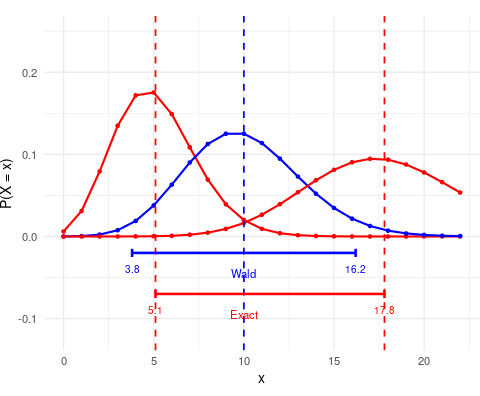
\includegraphics[width=0.64\textwidth]{figures/11-poisson-confidence-intervals.png}
  \caption{Poisson 均值的 Wald 区间与等尾区间（R 绘制）}
  \label{fig:ch11:poisson-ci}
\end{figure}


\end{example}

一种直接的 Bootstrap 方法，称作``\textbf{\emph{正态 Bootstrap 区间}} (normal-bootstrap interval)''，也就是把标准误交给 Bootstrap 估计。用 $B$ 次 Bootstrap 得到 $\widehat\theta_n^{*(1)},\ldots,\widehat\theta_n^{*(B)}$，令 \[ \bar\theta^* =\frac1B\sum_{b=1}^B\widehat\theta_n^{*(b)},\qquad \widehat{\mathrm{se}}_{\mathrm{boot}} =\left\{\frac1{B-1}\sum_{b=1}^B (\widehat\theta_n^{*(b)}-\bar\theta^*)^2\right\}^{1/2} \]正态 Bootstrap 区间为 \[ C_n^{\text{normal boot}} =\left[ \widehat\theta_n-z_{1-\alpha/2}\widehat{\mathrm{se}}_{\mathrm{boot}},\, \widehat\theta_n-z_{\alpha/2}\widehat{\mathrm{se}}_{\mathrm{boot}} \right] \]不过这只是改进了均值和方差 (标准误) 的估计值，仍然是在利用对称的正态分布，没有很好地反映出诸如偏态等高阶信息。

接下来，我们介绍三种进一步的 Bootstrap 置信区间技术，对应三种不同的根 $R(X;\theta)$ 选取策略：
\[\begin{array}{|c|c|c|} \hline \textbf{根} & \textbf{Bootstrap 对应量} & \textbf{区间类型}\\ \hline \widehat\theta_n-\theta & \widehat\theta_n^*-\widehat\theta_n & \text{基础 Bootstrap}\\ \widehat\theta_n & \widehat\theta_n^* & \text{百分位数 (percentile)}\\ \frac{\widehat\theta_n-\theta_0}{\widehat{\mathrm{se}}_n }& \frac{\widehat\theta_n^*-\widehat\theta_n}{\widehat{\mathrm{se}}_n^*} &\text{百分位数-$t$ (percentile-$t$)}\\\hline \end{array}\]
\subsection{基础 Bootstrap 置信区间}

考虑``中心化根''
\[
R_n(\theta_0):=\widehat\theta_n-\theta_0,\qquad R_n^*:=\widehat\theta_n^*-\widehat\theta_n.
\]

令 $r_p^*$ 是 $R_n^*$ 在条件概率 $P^*$ 下的 $p$ 分位数，即
\[r_p^* = \inf\{x:P^*(R_n^*\le x)\ge p\}\]
在实践中，用 $\widehat\theta_n^{*(1)}-\widehat\theta_n,\dots,\widehat\theta_n^{*(B)}-\widehat\theta_n$ 这 $B$ 个数的 $p$ -分位数来代替 $r_p^*$ 。

若 $R_n^*$ 对 $R_n$ 的近似可靠，则
\[P(r_{\alpha/2}^*\le \widehat\theta_n-\theta_0 \le r_{1-\alpha/2}^*)\approx 1-\alpha\]
求解 $\theta_0$ 得到
\[C_n^{\mathrm{basic}} =\left[ \widehat\theta_n-r_{1-\alpha/2}^*,\, \widehat\theta_n-r_{\alpha/2}^* \right]\]
若令 $q_p^*$ 表示 $\widehat\theta_n^*$ 自己的条件 $p$ 分位数，即
\[q_p^* = \inf\{x:P^*(\widehat\theta_n^*\le x)\ge p\}\]
则 $r_p^*=q_p^*-\widehat\theta_n$，同一个区间也可写成
\[C_n^{\mathrm{basic}} =\left[ 2\widehat\theta_n-q_{1-\alpha/2}^*,\, 2\widehat\theta_n- q_{\alpha/2}^* \right]\]
这种方法称作``\textbf{\emph{基础 Bootstrap 置信区间}} (basic bootstrap confidence interval )''。其思想是：

\begin{itemize}
\tightlist
\item
  若 Bootstrap 统计量 $\widehat\theta_n^*$ 高出 $\widehat\theta_n$ ，则说明 $\widehat\theta_n$ 很可能也高出真实参数 $\theta_0$ 。上分位数 $q_{1-\alpha/2}^*$ 描述的是``估计量可能高出中心多少''，因此当它较高时，需要让置信区间左端点往下拉；
\item
  同理，若 Bootstrap 统计量 $\widehat\theta_n^*$ 低于 $\widehat\theta_n$ ，则说明 $\widehat\theta_n$ 可能低于 $\theta_0$ 。下分位数 $q_{\alpha/2}^*$ 描述了``估计量可能低出中心多少''，当它越低时，需要把置信区间右端点向上拉。
\item
  需要注意的是，这种方法对参数的尺度比较敏感。
\end{itemize}

\subsection{百分位 Bootstrap}

\textbf{\emph{百分位区间}} (percentile interval) 直接取 Bootstrap 统计量 $\widehat\theta_n^*$ 的分布计算分位数，令
\[F_n^*(t)=P^*(\widehat\theta_n^*\le t), \qquad q_p^*={F_n^*}^{-1}(p)\]
在实践中，以 $\frac1B\sum_{b=1}^B\mathbb I\Big(\widehat\theta_n^{*(b)}\le t\Big)$ 来代替 $F_n^*(t)$ 。

那么一个 $1-\alpha$ 百分位区间为
\[C_n^{\mathrm{perc}}=\left[q_{\alpha/2}^*,q_{1-\alpha/2}^*\right]\]
也可以写成
\[
C_n^{\mathrm{perc}}
=\left\{\theta:\frac\alpha2\le F_n^*(\theta)\le 1-\frac\alpha2\right\}.
\]
这种方法思路很直接，就是用 Bootstrap 分布来找置信区间；直觉上，诸如偏度等高阶性质，可以体现在 Bootstrap 分布的形状当中，因此百分位区间也可以适应这一点。

如下是 \cite{efronhastie2016} 第 11.2 节的例子，数据原于 22 名学生分别参加两门课程考试的成绩，样本相关系数 $\widehat\theta_n=0.498$ 的取值，使用 $B=2000$ 次经验分布重抽样得到相关系数重复值，用这些数据的 $0.025$ 和 $0.975$ 分位数得到 $[0.118,0.758]$ 的百分位区间。

从图~\ref{fig:ch11:percentile-interval} 中可以明显看出 Bootstrap 统计量分布左偏，并反映到了百分位数区间的端点上：它在 $\widehat\theta_n$ 左侧的部分较长、右侧的部分较短；换言之，百分位区间是允许不对称的，这相比 Wald 置信区间是一个改进。

\begin{figure}[htbp]
  \centering
  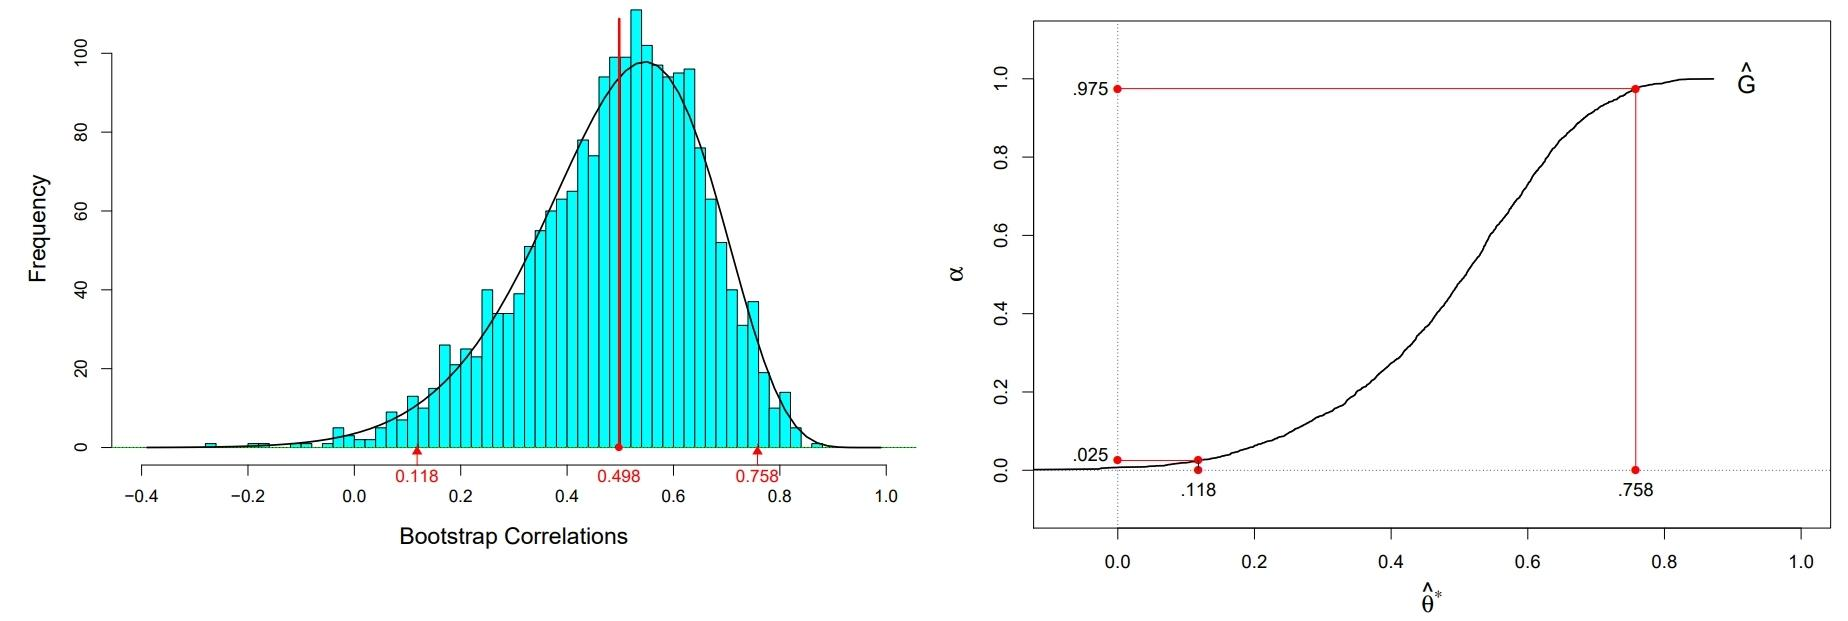
\includegraphics[width=0.94\textwidth]{figures/11-percentile-interval.png}
  \caption{相关系数的 Bootstrap 分布与百分位区间。图片来自 \cite{efronhastie2016}, \S11.2}
  \label{fig:ch11:percentile-interval}
\end{figure}

百分位区间的一个优点是，它在单调变换下保持不变性，这是说，若对参数空间作变换 $\theta\mapsto g(\theta)$ ，且 $g$ 严格递增，则 $g(\widehat\theta_n^*)$ 的 $\gamma$ 分位数就是 $g(q_\gamma^*)$。所以对 $\theta$ 做出的百分位区间，经过 $g$ 变换后，正是对 $g(\theta)$ 直接做百分位区间的结果。

例如上述相关系数的例子中，我们知道 Fisher 变换会把相关系数变到
\[\varphi=\frac12\log\frac{1+\theta}{1-\theta}\]
的尺度上做近似正态推断（见第~\ref{ch:delta-method}~章例~\ref{ex:ch5:fisher-z}）；百分位方法没有显式寻找这样的变换 $\varphi$，仅通过单调变换不变性便复现了这种尺度选择。本文介绍的其他两种 Bootstrap 区间一般不具有这种性质。

一阶正确性的推导非常容易：假设存在 $a_n\to\infty$，使得
\[a_n(\widehat\theta_n-\theta_0)\overset{\rm d}\to Z\]
其中 $Z$ 有\emph{连续且对称的分布函数}， $p$ 分位数记为 $z_p$。那么，若 Bootstrap 能够达到一阶正确：
\[\sup_x\left| P^*(a_n(\widehat\theta_n^*-\widehat\theta_n)\le x) -P(Z\le x) \right|\overset{P}\to 0\]
则
\[a_n(q_p^*-\widehat\theta_n)\overset{P}\to z_p\]
利用
\[\begin{aligned}  &q_{\alpha/2}^*\le \theta_0\le q_{1-\alpha/2}^*\\ \iff\ & a_n(q_{\alpha/2}^*-\widehat\theta_n) \le -a_n(\widehat\theta_n-\theta_0) \le a_n(q_{1-\alpha/2}^*-\widehat\theta_n)\end{aligned}\]
和 $Z$ 的对称性，取极限得到
\[P(\theta_0\in C_n^{\mathrm{perc}})\to P(z_{\alpha/2}\le -Z\le z_{1-\alpha/2}) =1-\alpha,\quad \text{ 当 }n\to\infty\]
不过，我们无法保证二阶准确性：$\widehat\theta_n$ 的分布通常不会是枢轴量，它依赖未知尺度、偏度、偏差和讨厌参数等等。Edgeworth 展开一旦写到 $n^{-1/2}$ 项，这些依赖就会进入分布修正项（ $n^{-1/2}$ 阶项），Bootstrap 未必能把一阶修正项抵消掉，所以覆盖误差经常只有 $O(n^{-1/2})$。为了提高覆盖误差的准确性，当目标是更高阶的覆盖精度，通常需要学生化，或者引入 BCa 这类专门修正端点的办法。

\subsection{学生化 Bootstrap}

记
\[
T_n(\theta_0) =\frac{\widehat\theta_n-\theta_0}{\widehat{\mathrm{se}}_n},\quad T_n^* =\frac{\widehat\theta_n^*-\widehat\theta_n} {\widehat{\mathrm{se}}_n^*}.
\]

若 $c_p$ 是 $T_n(\theta_0)$ 的真实 $p$ 分位数，则
\[P(c_{\alpha/2}\le T_n(\theta_0)\le c_{1-\alpha/2})=1-\alpha\]
反解出 $\theta_0$ 的范围得到理想的置信区间
\[\left[ \widehat\theta_n-c_{1-\alpha/2}\widehat{\mathrm{se}}_n,\, \widehat\theta_n-c_{\alpha/2}\widehat{\mathrm{se}}_n \right]\]
由于 $c_p$ 不可得，因此用 $T_n^*$ 的分位数 $c_p^*={F_n^*}^{-1}(p)$ 估计之，其中 $F_n^*$ 是 $T_n^*$ 的 CDF；在实践中，用
\[
\frac{\widehat\theta_n^{*(1)}-\widehat\theta_n}{\widehat{\mathrm{se}}_n^{*(1)}},
\dots,
\frac{\widehat\theta_n^{*(B)}-\widehat\theta_n}{\widehat{\mathrm{se}}_n^{*(B)}}
\]
的 $p$ 分位数代替 $c_p^*$。学生化 Bootstrap 区间，也叫 \textbf{\emph{百分位-$t$ 区间}}，为
\[C_n^{\mathrm{stud}} =\left[ \widehat\theta_n-c_{1-\alpha/2}^*\widehat{\mathrm{se}}_n,\, \widehat\theta_n-c_{\alpha/2}^*\widehat{\mathrm{se}}_n \right]\]
学生化的好处是，它``比较接近枢轴量''；除以 $\widehat{\mathrm{se}}_n$ 能够消掉尺度的影响，从而使 Bootstrap 捕捉更高阶的信息。回顾本章定理~\ref{thm:ch11:second-order-accuracy}，在适当的光滑性条件下，Bootstrap 能够达到二阶准确：
\[\sup_x \left| P^*(T_n^*\leq x)-P(T_n(\theta_0)\leq x) \right| =O_P(n^{-1})\]
我们希望，Bootstrap 的二阶准确能够推出百分位- $t$ 区间的二阶准确，即
\[P\big(F_n^{*-1}(\alpha/2)\le T_n\le F_n^{*-1}(1-\alpha/2)\big)= 1-\alpha+O(n^{-1})\]
或者简化一些：$c_p^*-c_p=O_P(n^{-1})$ ，也就是说 Bootstrap 分布的准确性能够传导到 Bootstrap 分位数的准确性。这依赖分布函数在分位数处能够足够光滑；在适当光滑性条件满足的时候，这一结论是成立的，请见下一节的 Cornish-Fisher 展开 。

\begin{theorem}[百分位-t 区间的二阶准确]\label{thm:ch11:percentile-t-second-order}

设标量参数 $\theta_0=\theta(P)$ 有估计量 $\widehat\theta_n$，且如下条件满足

\begin{itemize}
\tightlist
\item
  标准误估计满足 $\widehat{\mathrm{se}}_n/\mathrm{se}\overset P\to1$ ，其中 $\mathrm{se}>0$ ；
\item
  学生化统计量 $T_n$ 的分布函数 $F_n(x)=P(T_n\le x)$ 在分位数 $c_{\alpha/2}$ 和 $c_{1-\alpha/2}$ 附近有连续且有界的密度，且该密度在这两个点附近有正下界；
\item
  定理~\ref{thm:ch11:second-order-accuracy} 的光滑性条件成立，包括足够高阶矩存在，且 Edgeworth 二阶展开的 Cramér 条件成立。（此时 Bootstrap 统计量 $T_n^*$ 对 $T_n$ 具有二阶准确性： $\sup_x\left| P^*(T_n^*\le x)-P(T_n\le x) \right|= O_P(n^{-1})$ 。）
\end{itemize}

那么百分位-t 区间满足二阶准确性：
\[P\big(\theta_0\in C_n^{\text{stud}}\big)= 1-\alpha+O(n^{-1})\]
\end{theorem}

\subsection{Cornish-Fisher 展开}
\label{sub:ch11b:cornish-fisher}

定理~\ref{thm:ch11:percentile-t-second-order} 所依赖的结论里，唯一没有完整证明的理论是 Bootstrap 分位数的误差逼近，我们在本节就来进行证明。假设 Edgeworth 展开已经给出了某个 CDF $F_n(x)$ 满足，
\[F_n(x)=\Phi(x)+n^{-1/2}p_1(x)\varphi(x)+n^{-1}p_2(x)\varphi(x)+\cdots\]
我们希望从中反解 $p$ 分位数 $F_n^{-1}(p)$ 能有一个类似的渐近展开形式，形如
\[F_n^{-1}(p)=z_p+n^{-1/2}a_1(z_p)+n^{-1}a_2(z_p)+\cdots\]
其中 $z_p=\Phi^{-1}(p)$ 是标准正态的 $p$ 分位数。

这个反解过程本质上就是逐阶 Taylor 展开，接下来我们简要推导一下二阶的情形。

记 $\epsilon = n^{-1/2}$。考虑一族分布函数 $F_\varepsilon$，它们在标准正态分位数 $z_p$ 的一个邻域内满足一致的 Edgeworth 展开

\begin{equation}
\label{eq:ch11b:tag-6}
F_\epsilon(x) = \Phi(x) + \epsilon\, p_1(x)\varphi(x) + \epsilon^2 p_2(x)\varphi(x) + O(\epsilon^3)
\end{equation}

再假设在该邻域内

\begin{itemize}
\tightlist
\item
  $p_1,p_2$ 二阶连续可微；
\item
  $F_\epsilon$ 具有密度 $F_\epsilon'$ ；
\item
  对充分小的 $\varepsilon$ 存在正常数 $\eta,c$ 使得$\inf_{|x-z_p|\le \eta} F_\epsilon'(x) > c$这保证在 $z_p$ 附近反函数存在且 Lipschitz 连续。
\end{itemize}

我们的目标是对分位数 $x_{p,\epsilon}:=F_\epsilon^{-1}(p)$ 求出形如
\[x_{p,\epsilon} = z_p + \epsilon A + \epsilon^2 B + O(\epsilon^3)\]
的展开式，其中 $A,B$ 是待定的系数。记 $\delta = x - z_p = \epsilon A + \epsilon^2 B$，在 $z_p$ 处展开 $\Phi,\phi,p_1,p_2$：
\[\begin{aligned} \Phi(z_p+\delta) &= \Phi(z_p) + \varphi(z_p)\delta - \frac12 z_p \varphi(z_p)\delta^2 + O(\delta^3)\\ \varphi(z_p+\delta) &= \varphi(z_p)\bigl(1 - z_p\delta + O(\delta^2)\bigr) \end{aligned}\]\[\begin{aligned} p_1(z_p+\delta) &= p_1(z_p) + p_1'(z_p)\delta + O(\delta^2) \\ p_2(z_p+\delta) &= p_2(z_p) + O(\delta) \end{aligned}\]
然后逐项代入 式~\eqref{eq:ch11b:tag-6}。

\begin{itemize}
\tightlist
\item
  对 $\Phi(x)$ 项：
\end{itemize}
\[\begin{aligned} \Phi(x)=p+\varphi(z_p)\delta - \frac12 z_p \varphi(z_p)\delta^2  \end{aligned}\]
再将 $\delta = \epsilon A + \epsilon^2 B$ 代入，得到
\[\begin{aligned} \Phi(x)=p+ \varphi(z_p)(\epsilon A + \epsilon^2 B)-\frac12 z_p\varphi(z_p) \epsilon^2 A^2 + O(\epsilon^3) \end{aligned}\]
\begin{itemize}
\tightlist
\item
  对 $\epsilon$ 阶项：
  \[  \begin{aligned} \epsilon\, p_1(x)\varphi(x) &= \epsilon\, \varphi(z_p+\delta)\bigl(p_1(z_p)+p_1'(z_p)\delta + O(\delta^2)\bigr) \\ &= \epsilon\,\varphi(z_p)\bigl(1 - z_p\delta + O(\delta^2)\bigr) \bigl(p_1(z_p)+p_1'(z_p)\delta + O(\delta^2)\bigr) \\ &= \epsilon\,\varphi(z_p)\Bigl( p_1(z_p) + \delta\bigl(p_1'(z_p)-z_p p_1(z_p)\bigr) \Bigr) + O(\epsilon\delta^2). \end{aligned}
  \]  代入 $\delta = \epsilon A+O(\epsilon^2)$，我们得到
  \[  \epsilon\, p_1(x)\varphi(x) = \varphi(z_p)\Bigl( \epsilon p_1(z_p) + \epsilon^2 A\bigl(p_1'(z_p)-z_p p_1(z_p)\bigr) \Bigr) + O(\epsilon^3).
  \]\item
  对 $\epsilon^2$ 阶项：
  \[
  \epsilon^2 p_2(x)\varphi(x) = \epsilon^2 p_2(z_p)\varphi(z_p) + O(\epsilon^3).
  \]
\end{itemize}

将上面三部分加起来，则式~\eqref{eq:ch11b:tag-6} 可改写成：
\[\begin{aligned} F_\epsilon(x) - p &= \varphi(z_p)(\epsilon A + \epsilon^2 B)-\frac12 z_p\varphi(z_p) \epsilon^2 A^2 \\ &\quad + \varphi(z_p)\Bigl( \epsilon p_1(z_p) + \epsilon^2 A\bigl(p_1'(z_p)-z_p p_1(z_p)\bigr) \Bigr) \\ &\quad + \epsilon^2 p_2(z_p)\varphi(z_p) + O(\epsilon^3)\\ &= \varphi(z_p)\Bigl( \epsilon\bigl(A + p_1(z_p)\bigr) \\ &\quad +\epsilon^2\Bigl( B - \frac12 z_p A^2 + A\bigl(p_1'(z_p)-z_p p_1(z_p)\bigr) + p_2(z_p) \Bigr) \Bigr) + O(\epsilon^3). \end{aligned}\]选取 $A,B$ 使得 $F_\epsilon(x)=p+O(\epsilon^3)$，即上式中 $\epsilon$ 和 $\epsilon^2$ 的系数为零。

\begin{itemize}
\tightlist
\item
  一阶项：$A + p_1(z_p) = 0$，立即得到 \[A = -p_1(z_p)\]\item
  二阶项：代入 $A$，令 $\epsilon^2$ 的系数为零：
\end{itemize}
\[\begin{aligned} & B = \frac12 z_p A^2 - A\bigl(p_1'(z_p)-z_p p_1(z_p)\bigr) - p_2(z_p)\\ \implies &B= p_1(z_p)p_1'(z_p) - \frac12 z_p\, p_1(z_p)^2 - p_2(z_p) \end{aligned}\]
由此我们得到一个``近似分位数''：

\begin{equation}
\label{eq:ch11b:tag-7}
\widetilde{x}_{p,\epsilon} = z_p - \epsilon p_1(z_p) + \epsilon^2\Bigl( p_1(z_p)p_1'(z_p) - \frac12 z_p p_1(z_p)^2 - p_2(z_p) \Bigr)
\end{equation}

它满足 $F_\epsilon(\widetilde{x}_{p,\epsilon}) = p + O(\epsilon^3)$。

用 $\widetilde{x}_{p,\epsilon} \to z_p$（当 $\epsilon\to0$），真实分位数 $x_{p,\epsilon}$ 也落在该邻域内。由微分中值定理，
\[c\,|x_{p,\epsilon} - \widetilde{x}_{p,\epsilon}|\le |F_\epsilon(x_{p,\epsilon}) - F_\epsilon(\widetilde{x}_{p,\epsilon})|=|\,p - F_\epsilon(\widetilde{x}_{p,\epsilon})\,|=O(\epsilon^3)\]
即 $x_{p,\epsilon} = \widetilde{x}_{p,\epsilon} + O(\epsilon^3)$ ；所以式~\eqref{eq:ch11b:tag-7} 就是我们想要的展开，它称作 \textbf{\emph{Cornish-Fisher 展开}} 。

写作定理：

\begin{theorem}[二阶 Cornish-Fisher 展开]

令 $z_p=\Phi^{-1}(p)$，设分布函数 $F_n$ 在 $z_p$ 附近密度存在有正的下界，且 $F_n$ 有二阶 Edgeworth 展开
\[F_n(x)=\Phi(x)+n^{-1/2}p_1(x)\varphi(x)+n^{-1}p_2(x)\varphi(x)+O(n^{-3/2})\]
其中余项在 $z_p$ 的某邻域内一致成立，且 $F_n$ 在该邻域内严格递增。那么， $F_n^{-1}(p)$ 满足
\[F_n^{-1}(p) = z_p -n^{-1/2}p_1(z_p) +n^{-1} \left( p_1(z_p)p_1'(z_p) -\frac12 z_p p_1(z_p)^2 -p_2(z_p) \right) +O(n^{-3/2})\]
简而言之概括：只要分布函数在 $p$ 分位数附近足够光滑，那么 Edgeworth 展开有多精确， Cornish-Fisher 展开就有多精确。

将之用于 Bootstrap 分布 ${F_n^*}^{-1}(p)$ ：在定理~\ref{thm:ch11:second-order-accuracy} 的条件下， $T_n^*$ 和 $T_n(\theta_0)$ 有 Edgeworth 展开：
\[\begin{aligned} P(T_n(\theta_0)\le x) &= \Phi(x)+n^{-1/2}p_1(x;P)\varphi(x)  +O_P(n^{-1})\\ P^*(T_n^*\le x) &= \Phi(x)+n^{-1/2}p_1(x;\mathbb P_n)\varphi(x) +O_P(n^{-1}) \end{aligned}\]
且 $p_1(x;P)-p_1(x;\mathbb P_n)=O_P(n^{-1/2})$ ，那么 Cornish-Fisher 展开给出
\[\begin{aligned} & \begin{aligned} c_p &= z_p-n^{-1/2} p_1(z_p;P) +O(\epsilon^2)\\ c^*_p &= z_p-n^{-1/2}p_1(z_p;\mathbb P_n) +O(\epsilon^2) \end{aligned}\\ \implies\ & c_p-c_p^*=-n^{-1/2}\big(p_1(z_p;P) -p_1(z_p;\mathbb P_n) \big)+O_P(n^{-1}) =O_P(n^{-1}) \end{aligned}\]
这就是定理~\ref{thm:ch11:percentile-t-second-order} 所需要的结论。

\end{theorem}

这种技术来自于 \cite{hall1986}；读者也可以参考 \cite{hall1992} 一书。

\subsection{偏差校正与 BCa 区间}

众所周知，Bootstrap 也能估计偏差：
\[\widehat{\mathrm{bias}}_{\mathrm{boot}} =\mathbb E^*[\widehat\theta_n^*]-\widehat\theta_n \approx \frac1B\sum_{b=1}^B\widehat\theta_n^{*(b)} -\widehat\theta_n\]
因此对一个点估计 $\widehat\theta_n$ ，我们可以写出它的偏差校正：
\[\widehat\theta_n^{\mathrm{bc}} =\widehat\theta_n-\widehat{\mathrm{bias}}_{\mathrm{boot}}\]
当然，点估计的偏差校正不能自动变成好的置信区间。我们要的实际上是校正``中位偏差 (median bias)''：若 Bootstrap 分布已经围绕 $\widehat\theta_n$ 是对称的，那么应有 $P^*(\widehat\theta_n^*\le \widehat\theta_n)\approx \tfrac12$ 。实际数据会告诉我们这个比例是否偏离 $\tfrac12$：令
\[
\widehat p_0 = P^*(\widehat\theta_n^*\le \widehat\theta_n) \approx \frac1B\sum_{b=1}^B\mathbb I\Big(\widehat\theta_n^{*(b)}\le \widehat\theta_n\Big).
\]

并定义偏差校正常数
\[\widehat z_0:=\Phi^{-1}(\widehat p_0)\]
$\widehat z_0=0$ 对应 Bootstrap 分布以 $\widehat\theta_n$ 为中位中心；$\widehat z_0<0$ 表示少于一半的 Bootstrap 重复值落在 $\widehat\theta_n$ 左边，Bootstrap 重复值整体偏高，区间端点通常要往低调整；$\widehat z_0>0$ 则相反。

BC-百分位 (BC-percentile) 方法直接修改百分位区间的概率截点。仍记 $F_n^*(t)=P^*(\widehat\theta_n^*\le t)$ 、 $q_p^*=(F_n^*)^{-1}(p)$ 、 $z_p=\Phi^{-1}(p)$ ；对名义水平 $p$ ，BC-百分位方法使用 $\Phi(2\widehat z_0+z_{p})$ 作为新的 Bootstrap 分位数水平，那么名义 $1-\alpha$ 的 BC-百分位区间为
\[C_n^{\text{BC}}=\Big[{F_n^*}^{-1}(\Phi(2\widehat z_0+z_{\alpha/2})),{F_n^*}^{-1}(\Phi(2\widehat z_0+z_{1-\alpha/2}))\Big]\]
简而言之： 若 $\widehat z_0\ne0$，说明 Bootstrap 分布的中位中心没有落在 $\widehat\theta_n$，BC-百分位把正态分位数刻度以 $\widehat z_0$ 为中心作平移校正， $z_p$ 被替换为 $2\widehat z_0+z_p$ 。若 $\widehat z_0=0$，BC-百分位退回普通百分位区间。

BC-百分位仍然只校正中位偏差。若标准误在参数尺度上变化，单靠 $\widehat z_0$ 不够。BCa 方法在 BC 的基础上引入加速常数 $\widehat a$ ，通过额外的影响函数或者 jackknife 方法从样本中计算获得，然后以 $\Phi\left( \widehat z_0+ \frac{\widehat z_0+z_p} {1-\widehat a(\widehat z_0+z_p)} \right)$ 作为新的 Bootstrap 分位数水平。可以说 BCa 使用了多达三重的校正：分位数 Bootstrap 校正分布近似、 $\widehat z_0$ 校正偏差、 $\widehat a$ 校正标准误；这也使得该方法能够达到二阶的准确。

我们对此不作更多介绍，可以参考 \cite{efron1987}。

\begin{example}[指数分布的置信区间比较]\label{ex:ch11:exponential}

设从指数分布 (尺度参数化) $\mathrm{Exp}(\theta)$ 中抽取出 $n=5$ 的样本，记样本均值为 $\widehat\theta$ ，图~\ref{fig:ch11:ci-exponential} 展示了精确置信区间、分位数区间、BC、BCa 四种置信区间的左右端点 $L\widehat\theta,U\widehat\theta$ ，以及各自的尾部面积 $P(L\widehat\theta>\theta)$ 和 $P(U\widehat\theta<\theta)$(图中称作错误率，\%) 。

\begin{figure}[htbp]
  \centering
  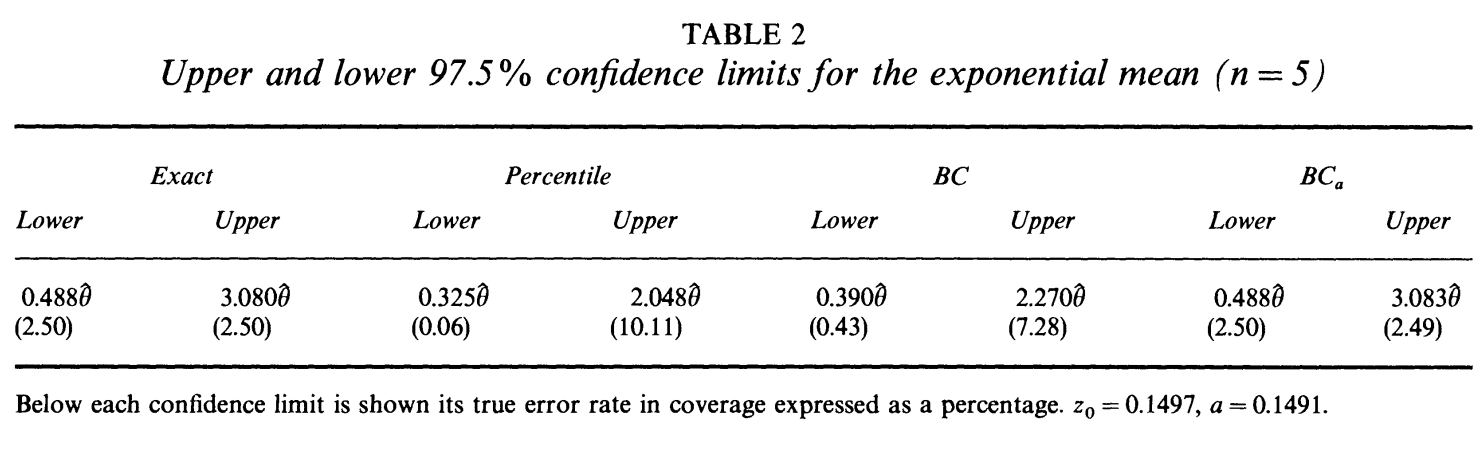
\includegraphics[width=0.96\textwidth]{figures/11-confidence-interval-comparison.png}
  \caption{指数分布均值的四种置信区间比较。图片来自 \cite{diciccioromano1988}}
  \label{fig:ch11:ci-exponential}
\end{figure}

其中，

\begin{itemize}
\tightlist
\item
  精确的 95\% 置信区间可以利用枢轴量 $\tfrac{2n\widehat\theta}{\theta}\sim\chi_{2n}^2$ 得出： $\left[\frac{2n\widehat\theta}{\chi^2_{2n}(0.975)},\frac{2n\widehat\theta}{\chi^2_{2n}(0.025)}\right]$ ；
\item
  使用参数 Bootstrap ，则应用 $\mathrm{Exp}(1/\widehat\theta)$ 代替样本分布；本例中不需要真的 Monte Carlo 重抽样，只需要再次利用枢轴量，即可用 χ² 分布的分位数得到各 Bootstrap 区间。例如，令 $q_p$ 代表 $\chi^2_{2n}$ 的 $p$ 分位数，则百分位区间为 $\left[\tfrac{q_{0.025}}{2n}\widehat\theta,\tfrac{q_{0.975}}{2n}\widehat\theta\right]$ 。
\end{itemize}

下面是一个稍微复杂一些的例子，取 $X\sim \mathrm{Exp}(1/\eta^1)$ 、 $Y\sim\mathrm{Gamma}(c,1/\eta^2)$ ， $\theta=\eta^2/\eta^1$ ，其中 $c=0.4$ 。仍取 $n=5$ 个样本， $\widehat\theta=\frac{\widehat\eta^2}{\widehat\eta^1}=\frac{c\sum_{j=1}^5 X_j}{\sum_{j=1}^5Y_j}$ 是 $\eta^2$ 和 $\eta^1$ 的 MLE 之比。四种置信区间的比较见图~\ref{fig:ch11:ci-ratio}。

\begin{figure}[htbp]
  \centering
  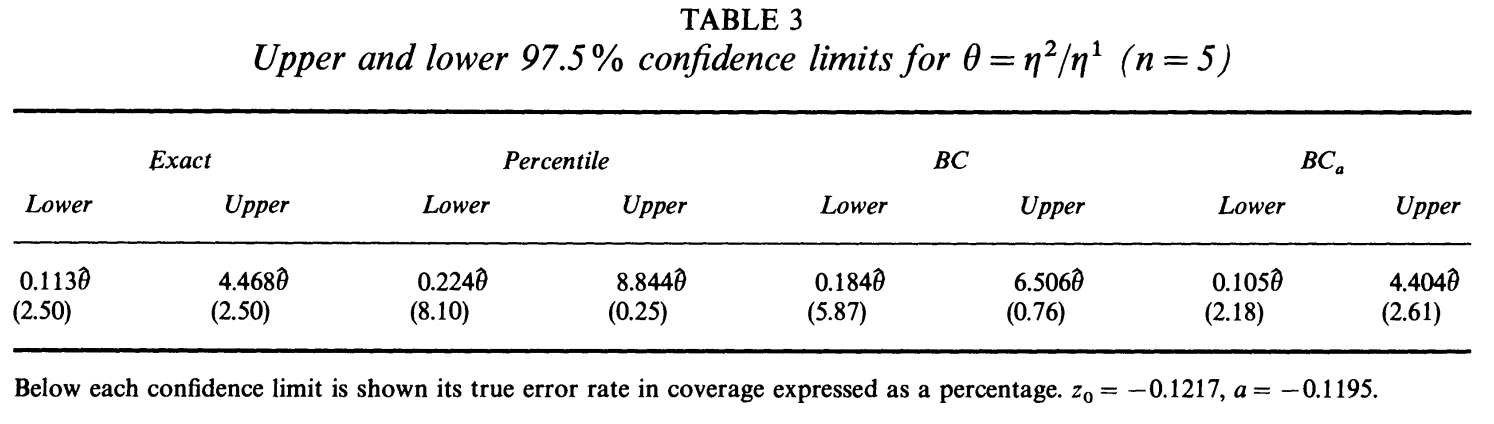
\includegraphics[width=0.96\textwidth]{figures/11-ratio-confidence-interval-comparison.png}
  \caption{两参数比值的四种置信区间比较。图片来自 \cite{diciccioromano1988}}
  \label{fig:ch11:ci-ratio}
\end{figure}

精确的 95\% 置信区间可以利用枢轴量 $\tfrac{\widehat\theta}{\theta}\sim F_{2n,2nc}$ 算出。

这两个例子中，普通百分位区间和 BC 区间的两侧错误率明显不平衡，而 BCa 区间几乎与精确区间一致。


\end{example}

\section{关于 Bootstrap 的补充}

\subsection{失效}

Bootstrap 不是在任何情况下都可以随便用的------虽然它在很多时候都非常方便且好用，但其\emph{正当性必须由其渐近结构来保证}。如果正则条件不满足，完全可以构造 Bootstrap 失效的例子。这些例子包括

\begin{itemize}
\tightlist
\item
  统计泛函 $\theta(P)$ 不光滑；
\item
  $\widehat\theta_n$ 逼近 $\theta_0$ 的速率不是标准的 $O_P(n^{-1/2})$ ，那么重抽样样本与原始样本量相同的`` $n$ -out-of- $n$ '' Bootstrap 是不适用的；
\item
  参数落在支撑集合的边界上，或者统计量依赖于分布极值或支撑边界，如样本极值；见下面的例~\ref{ex:ch11:extreme}。
\item
  对相依数据使用 i.i.d. Bootstrap：例如 $X_j$ 是时间序列，那么从 $\mathbb P_n$ i.i.d. 抽样显然会破坏自相关结构。
\item
  模型选择或者 post-selection 估计量。
\end{itemize}

% \href{https://stats.stackexchange.com/questions/9664/what-are-examples-where-a-naive-bootstrap-fails}{What are examples where a ``naive bootstrap'' fails? - Cross Validated}

\cite{chernick2011} 一书的第 9 章就深入讨论了各种 Bootstrap 失效的情形。我们举一个最简单的例子：

\begin{example}[样本极值]
\label{ex:ch11:extreme}
设
\[X_1,\ldots,X_n\sim \mathcal{U}(0,\theta)\quad \text{i.i.d.}, \qquad \widehat\theta_n=X_{(n)}=\max_i X_i\]
不难证明 $\widehat\theta_n$ 真实极限为
\[n(\theta-X_{(n)})\overset{\rm d}\to \mathrm{Exp}(\theta)\]
Bootstrap 最大值 $X_{(n)}^*$ 从原样本中重抽；以原始数据为条件，Bootstrap 样本包含原最大值 $X_{(n)}$ 的概率是
\[P^*(X_{(n)}^*=X_{(n)}) =1-\left(1-\frac1n\right)^n \to 1-e^{-1}\]
因此 $n\big(X_{(n)}-X_{(n)}^*\big)$ 在 $0$ 处保留一个约 $1-e^{-1}$ 的原子概率，而真实极限是连续的指数分布。一个带固定的原子概率的条件分布，显然是不可能依分布收敛到指数分布的。


\end{example}

例~\ref{ex:ch11:extreme} 的问题在于，经验分布很难捕捉极值 $X_{(n)}$ 这一信息，每次重抽样可能完全抽不到 $X_{(n)}$ 。如果从参数的角度出发，$\theta$ 位于支撑集的边界上，也可视作造成问题的原因；若将 $\theta$ 视作统计泛函 $\mathcal U(0,\theta)\mapsto \theta$ ，它在某些方向上甚至不存在有限的 Gâteaux 导数，自然不会满足定理~\ref{cor:ch11:functional-delta-normality} 的条件。

还有要注意的是，就算 Bootstrap 能满足一阶正确性，二阶准确性也可能失效。回顾定理~\ref{thm:ch11:second-order-accuracy}，要保证 Bootstrap 二阶准确性，至少需要

\begin{itemize}
\tightlist
\item
  统计量足够光滑；
\item
  有足够阶矩存在；
\item
  Edgeworth 展开所需的 Cramér 条件；
\item
  如果 Bootstrap 过程需估计讨厌参数，它们必须有足够好的相合估计；
\item
  统计量是渐近枢轴量。
\end{itemize}

总之，一阶有效 $\nRightarrow$ 二阶准确。

\subsection{变体}

由于上述各种例外情况，我们介绍的一般 Bootstrap 也有很多不同的变体；关键问题是：如何使用现有的样本得到一个``能够很好近似目标样本分布''的分布，而这基本都是从重抽样方案出发进行改进。如下：
\[\begin{array}{|c|c|}\hline \textbf{问题结构} & \text{Bootstrap 变体}\\ \hline \text{有可信的参数模型 }P_\theta & \text{参数 Bootstrap}\\ \hline \text{有光滑的密度} & \substack{\displaystyle\text{光滑 Bootstrap}\\ \displaystyle\text{(Smoothed Bootstrap)}}\\ \hline \text{非标准收敛速率/边界} & \substack{\displaystyle \text{ $m$-out-of-$n$ Bootstrap,}\\ \displaystyle\text{子采样 (Subsampling)}}\\ \hline \text{异方差回归}& \text{Wild Bootstrap}\\ \hline \text{时间序列或空间相关} & \substack{\displaystyle\text{分块 Bootstrap}\\ \displaystyle\text{(Block Bootstrap)}}\\ \hline \text{高维经验过程} & \substack{\displaystyle\text{乘子 Bootstrap}\\ \displaystyle\text{(Multiplier Bootstrap)}}\\ \hline \end{array}\]
这些方法各自对应一种结构判断：

\begin{itemize}
\tightlist
\item
  参数 Bootstrap 已在本章前文介绍：如果参数族模型正确，那么参数 Bootstrap 往往能够得到效率更高的估计。
\item
  光滑 Bootstrap 类似：如果我们已知``目标样本分布有光滑的密度''，那么可以将重抽样的分布平滑一下，例如核平滑 (Kernel Smoothing)，再来用于近似目标分布，这样也可能提高估计效率，并且避免了``只能从已知样本中重抽样，导致经常抽出重复值''的问题。见 \cite{silvermanyoung1987}。
\item
  如果 $\widehat\theta_n$ 收敛于 $\theta$ 的速度比 $O_P(n^{-1/2})$ 更快，比如例~\ref{ex:ch11:extreme} 是按照 $O_P(n^{-1})$ 速度，那么就不能再简单地让重抽样样本与原始样本量相同，考虑 $\text{$m$-out-of-$n$}$ Bootstrap，每次重抽样只抽取 $m$ 次，其中 $m/n\to 0$ 、 $m\to\infty$ ，例如可以取 $m=\sqrt n$ 。这样，Bootstrap 样本的极端值行为与真实抽样更匹配。参数位于边界的情况同理。
\item
  子采样 (subsampling) 由 \cite{politisromano1994} 系统提出。简而言之，其思路是运行很多次重采样，采样次数 $m$ 远小于 $n$ （同样 $m/n\to 0$ 、 $m\to\infty$ ），但与 $\text{$m$-out-of-$n$}$ Bootstrap 不同的是，这里的重采样是\emph{无放回}的。子采样的正确性可以在非常弱的条件下成立，不需要 Bootstrap 那样的光滑性条件；对于有依赖的时间序列数据，子采样也可以使用，总之是一种比较强大的方法。进一步可参考 \cite{politisromanowolf1999}。
\item
  Wild Bootstrap 已在本章例~\ref{ex:ch11:wild-bootstrap} 中介绍。
\item
  如果数据存在序列相关或空间相关，独立重抽样会打乱相依结构，这种情况下可以用分块 Bootstrap。例如对平稳离散时间序列就把相邻 $l$ 个时间的 $X_t$ 放在同一个块中（允许块间重叠），然后以块为单位进行重抽样，再把重抽样块拼到一起，这种方法来自 \cite{kunsch1989}。
\item
  乘子 Bootstrap ( multiplier bootstrap) 的思想是生成辅助随机变量 $w_1,\dots,w_n$ ，从而构造随机加权的经验过程 $\mathbb G_n^wf=\frac1{\sqrt n}\sum_{j=1}^nw_j(f(X_j)-Pf)$ 。这个理论比较复杂，不多赘述。
\end{itemize}

最后，我们以一个 $\text{$m$-out-of-$n$}$ Bootstrap的例子作为结尾。

\begin{example}[$m$-out-of-$n$ 的极值例]
\label{ex:ch11:m-out-of-n}

设 $m\to\infty$，且 $m/n\to 0$。定义 bootstrap 统计量
\[T_{n,m}^* = m\big(X_{(n)}-X_{(m)}^*\big)\]
其中 $X_{(m)}^*$ 是从经验分布中有放回抽取 $m$ 个样本的最大值。显见， \[ P^*(T_{n,m}^*=0)=P^*\big(X_{(n)}=X_{(m)}^*\big)=1-\left(1-\frac1n\right)^m=\frac mn+o\left(\frac mn\right)\to 0 \]所以之前``在 0 处总存在原子概率''的问题完全被解决了。

对任意固定的 $t \ge 0$，
\[ \begin{aligned} P^*\bigl(T_{n,m}^* > t\bigr) &= P^*\left(X_{(m)}^* < X_{(n)} - \frac{t}{m}\right) \\ &= \left(\mathbb F_n\!\left(X_{(n)} - \frac{t}{m}\right)\right)^m \\ &=\left(1-\frac {N_{n,t}}n\right)^m \end{aligned} \]其中 $N_{n,t} := \#\left\{i : X_i > X_{(n)} - \tfrac{t}{m}\right\}$ 。

给定 $X_{(n)}$ 时，其余 $n-1$ 个样本点独立地服从 $\mathcal{U}(0, X_{(n)})$，落入区间 $\bigl(X_{(n)} - \frac{t}{m},\, X_{(n)}\bigr]$ 的概率为 $\tfrac{t/m}{X_{(n)}}$，因此
\[N_{n,t} - 1 \mid X_{(n)} \;\sim\; \mathrm{Binomial}\left(n-1,\; \frac{t}{m X_{(n)}}\right)\]
得
\[\begin{aligned} \mathbb{E}\left[\frac{m N_{n,t}}{n} \ \bigg|\  X_{(n)}\right] &=\frac{m}{n}+\frac{m(n-1)}{n}\frac{t}{m X_{(n)}} \overset P\to \frac{t}{\theta}\\  \mathrm{Var}\left[\frac{m N_{n,t}}{n} \ \bigg|\  X_{(n)}\right] &= \frac{m^2}{n^2}(n-1)\frac{t}{m X_{(n)}}\left(1-\frac{t}{m X_{(n)}}\right) = O\left(\frac{m}{n}\right) \to 0  \end{aligned}\]
这推出 $\tfrac{mN_{n,t}}{n}\overset{P}\to\tfrac t\theta$ ，利用这一点，以及 $\tfrac{N_{n,t}}{n}=O_{P}\left(\tfrac1m\right)$ ，最终得到
\[P^*\bigl(T_{n,m}^* > t\bigr) = \exp\!\left\{m\log\!\left(1 - \frac{N_{n,t}}{n}\right)\right\}=\exp\left\{-\frac {mN_{n,t}}{n}+O_{P}\left(\frac 1m\right)\right\} \overset{P}\longrightarrow e^{-t/\theta}\]
这就证明了 $T_{n,m}^*\overset{\rm d^*}\to\mathrm{Exp}(\theta)$ ，且由条件版本的 Pólya 定理，
\[\sup_x \bigl| P^*(T_{n,m}^* \le x) - P(\mathrm{Exp}(\theta) \le x) \bigr| \xrightarrow{P} 0\]
\end{example}

